\setchapterimage[6cm]{chapter/city/SanFrancisco_from_TwinPeaks_dusk_MC.jpg}
\setchapterpreamble[u]{\margintoc}
\chapter{From towns to cities with millions of inhabitants\protect\footnotemark}
\labch{city}

\footnotetext{\href{https://en.wikipedia.org/wiki/San_Francisco}{San Francisco} panorama from \href{https://en.wikipedia.org/wiki/Twin\_Peaks\_(San\_Francisco)}{Twin Peaks}. San Francisco is the city in \href{https://en.wikipedia.org/wiki/Northern\_California}{Northern California (United States of America)} where the \href{https://en.wikipedia.org/wiki/Wikimedia\_Foundation}{Wikimedia Foundation} is headquartered.
Author: \href{https://commons.wikimedia.org/wiki/File:SanFrancisco\_from\_TwinPeaks\_dusk\_MC.jpg}{Christian Mehlführer, WikiCommons / 2006 / Creative Commons Attribution License}. A part of the original file is presented. }

The chapter is devoted to the study of different types of cities corresponding to the four objects of Wikidata — "town", "city", "big city" and "city with millions of inhabitants". Using SPARQL queries to Wikidata, data on the number of instances of the objects under study were obtained and issues related to the "population" and "sister city" properties of these Wikidata objects were considered. The following tasks have been solved: calculation and analysis of the population of different types of cities; determination of the number of cities without sister cities; construction a list of cities ordered by the number of sister cities; finding the number of cities with a certain amount of sister cities; determination of the country with most sister cities; finding the closest neighbours of Russia. In conclusion, an assessment of the completeness of the data presented in Wikipedia and Wikidata is given, and the problems and difficulties that have arisen when studying objects of different types of cities are listed.

%%%%%%%%%%%%%%%%%%%%%%%%%%%%%%%%%%%%%%%%%%%%%%%%%%%%%%%
\section{Instances}

SPARQL queries for getting instances of the objects under study are presented below: \wdqName{town}{3957} (Listing \ref{lst:town}), \wdqName{city}{515} (Listing \ref{lst:city}), \wdqName{big city}{1549591} (Listing \ref{lst:big_city}), \wdqName{city with millions of inhabitants}{1637706} (Listing \ref{lst:city_million}). Additionally SPARQL query for getting instances of different types of cities have been constructed (Listing \ref{lst:different_city_types}).

\begin{lstlisting}[ language=SPARQL, 
                    caption={Instances of \wdqName{town}{3957}\\\hspace{\textwidth}
                        The result contains \num{13 800} towns in 2020.\\\hspace{\textwidth}
                        SPARQL query: \href{https://w.wiki/m3d}{w.wiki/m3d}
                        },
                    label=lst:town,
                    texcl 
                    ]
SELECT ?city ?cityLabel WHERE {
	?city wdt:P31 wd:Q3957. # instances of "town"
	SERVICE wikibase:label { bd:serviceParam wikibase:language "en" }
}
\end{lstlisting}%

\begin{lstlisting}[ language=SPARQL, 
                    caption={Instances of \wdqName{city}{515}\\\hspace{\textwidth}
                        The result contains \num{20 800} cities in 2017, 
                        \num{9 260} "Cities" in 2020.\\\hspace{\textwidth}
                        SPARQL query: \href{https://w.wiki/m3c}{w.wiki/m3c}
                        },
                    label=lst:city,
                    texcl 
                    ]
SELECT ?city ?cityLabel WHERE {
	?city wdt:P31 wd:Q515. # instances of "city"
	SERVICE wikibase:label { bd:serviceParam wikibase:language "en" }
}
\end{lstlisting}%

According to ProWD \wdqName{Singapore}{334} is the leader in terms of the number of properties (104 properties) among cities around the world. \wdqName{Novorossiysk}{15760} contains 31 properties. This is the maximum number of properties for Russian cities.

\begin{lstlisting}[ language=SPARQL, 
                    caption={Instances of \wdqName{big city}{1549591}\\\hspace{\textwidth}
                        The result contains 198 big cities in 2017, 
                        \num{3075} big cities in 2020.\\\hspace{\textwidth}
                        SPARQL query: \href{https://w.wiki/m3b}{w.wiki/m3b}
                        },
                    label=lst:big_city,
                    texcl 
                    ]
SELECT ?city ?cityLabel WHERE {
	?city wdt:P31 wd:Q1549591. # instances of "big city"    
	SERVICE wikibase:label { bd:serviceParam wikibase:language "en" }
}
\end{lstlisting}%

According to ProWD \wdqName{Singapore}{334} is the leader in terms of the number of properties (104 properties) among big cities around the world. \wdqName{Moscow}{649} contains 76 properties which is the maximum number for Russian big cities.

\begin{lstlisting}[ language=SPARQL, 
                    caption={Instances of \wdqName{city with millions of inhabitants}{1637706}\\\hspace{\textwidth}
                        The result contains 616 cities with millions of inhabitants in 2020.\\\hspace{\textwidth}
                        SPARQL query: \href{https://w.wiki/m3a}{w.wiki/m3a}
                        },
                    label=lst:city_million,
                    texcl 
                    ]
SELECT ?city ?cityLabel WHERE {
	?city wdt:P31 wd:Q1637706. # instances of "city 1000000+" 
	SERVICE wikibase:label { bd:serviceParam wikibase:language "en" }
}
\end{lstlisting}%

\begin{lstlisting}[ language=SPARQL, 
                    caption={Instances of different types of cities\\\hspace{\textwidth}
                        The result contains \num{26 751} instances of different types of cities in 2020.\\\hspace{\textwidth}
                        SPARQL query: \href{https://w.wiki/m3Y}{w.wiki/m3Y}
                        },
                    label=lst:different_city_types,
                    texcl 
                    ]
SELECT ?city ?cityLabel WHERE { # Selecting items which are ...
	{ ?city wdt:P31 wd:Q3957 } UNION # instances of "town"
	{ ?city wdt:P31 wd:Q515 } UNION # instances of "city"
	{ ?city wdt:P31 wd:Q1549591 } UNION # instances of "big city"
	{ ?city wdt:P31 wd:Q1637706 } # instances of "city 1000000+"                                
	SERVICE wikibase:label { bd:serviceParam wikibase:language "en" }
}
\end{lstlisting}%

%%%%%%%%%%%%%%%%%%%%%%%%%%%%%%%%%%%%%%%%%%%%%%%%%%%%%%%
\section{Population}

SPARQL queries for finding total population of objects under study instances are presented below: \wdqName{town}{3957} (Listing \ref{lst:population_town}), \wdqName{city}{515} (Listing \ref{lst:population_city}), \wdqName{big city}{1549591} (Listing \ref{lst:population_big_city}), \wdqName{city with millions of inhabitants}{1637706} (Listing \ref{lst:population_city_millions}).

\begin{lstlisting}[ language=SPARQL, 
                    caption={Population of towns\\\hspace{\textwidth}
                        The result contains \num{53304439} people in 2020.\\\hspace{\textwidth}
                        SPARQL query: \href{https://w.wiki/m3V}{w.wiki/m3V}
                        },
                    label=lst:population_town,
                    texcl 
                    ]
# Selecting total population of items which are ...
SELECT (SUM(?population_city) as ?sum) WHERE {                    
	SELECT (MAX(xsd:integer(REPLACE(STR(?population),"\\.",""))) 
						as ?population_city) ?city WHERE {
		?city wdt:P31 wd:Q3957.	# instances of "town"
		?city wdt:P1082 ?population # with filled property "population"                                  
	}
	GROUP BY ?city
}
\end{lstlisting}%

\begin{lstlisting}[ language=SPARQL, 
                    caption={Population of cities\\\hspace{\textwidth}
                        The result contains \num{1 133 560 167} people in 2020.\\\hspace{\textwidth}
                        SPARQL query: \href{https://w.wiki/m3T}{w.wiki/m3T}
                        },
                    label=lst:population_city,
                    texcl 
                    ]
# Selecting total population of items which are ...
SELECT (SUM(?population_city) as ?sum) WHERE {                    
	SELECT (MAX(xsd:integer(REPLACE(STR(?population),"\\.",""))) 
						as ?population_city) ?city WHERE {
		?city wdt:P31 wd:Q515. # instances of "city"
		?city wdt:P1082 ?population # with filled property "population"
	}
	GROUP BY ?city
}
\end{lstlisting}%

\begin{lstlisting}[ language=SPARQL, 
                    caption={Population of big cities\\\hspace{\textwidth}
                        The result contains \num{2 538 491 725} people in 2020.\\\hspace{\textwidth}
                        SPARQL query: \href{https://w.wiki/m3S}{w.wiki/m3S}
                        },
                    label=lst:population_big_city,
                    texcl 
                    ]
# Selecting total population of items which are ...
SELECT (SUM(?population_city) as ?sum) WHERE {                    
	SELECT (MAX(xsd:integer(REPLACE(STR(?population),"\\.",""))) 
						as ?population_city) ?city WHERE {
		?city wdt:P31 wd:Q1549591. # instances of "big city"
		?city wdt:P1082 ?population # with filled property "population"
	}
	GROUP BY ?city
}
\end{lstlisting}%

\begin{lstlisting}[ language=SPARQL, 
                    caption={Population of cities with millions of inhabitants\\\hspace{\textwidth}
                        The result contains \num{2 118 385 113} people in 2020.\\\hspace{\textwidth}
                        SPARQL query: \href{https://w.wiki/m3R}{w.wiki/m3R}
                        },
                    label=lst:population_city_millions,
                    texcl 
                    ]
# Selecting total population of items which are ...
SELECT (SUM(?population_city) as ?sum) WHERE {
	SELECT (MAX(xsd:integer(REPLACE(STR(?population),"\\.",""))) 
						as ?population_city) ?city WHERE {
		?city wdt:P31 wd:Q1637706. # instances of "city 1000000+"
		?city wdt:P1082 ?population # with filled property "population"
	}
	GROUP BY ?city
}
\end{lstlisting}%

Different countries use different characters as separators, such as point, comma, or space. As a result, the variants of representing the value of the \href{https://www.wikidata.org/wiki/Property:P1082}{population} property can also be different. Problems arise when using a point, because in Wikidata this character is the separator between the integer and decimal parts of a number. To disambiguate, \href{https://en.wikibooks.org/wiki/SPARQL/Expressions\_and\_Functions\#REPLACE}{REPLACE} function to remove the specified character should be used (Listings \ref{lst:population_town},   \ref{lst:population_city}, \ref{lst:population_big_city}, \ref{lst:population_city_millions}). This conversion does not affect the value itself, since the population is an integer, and the separators are used solely for ease of reading.

The \reftab{tab:population} shows a summary of the population of different types of cities, as well as the proportion of the population per type of city of the \href{https://en.wikipedia.org/wiki/World\_population}{world population}, which reached approximately 7,8 billion people in 2020.

\begin{table}[h]
  \centering
  \fontfamily{ppl}\selectfont
  \begin{tabular}{| l | r | r |}
    \toprule
   \multicolumn{1}{| c |}{City type} & \multicolumn{1}{p{0.25\textwidth} |}{\centering Population (million people)} & \multicolumn{1}{p{0.15\textwidth} |}{\centering \% of world} \\
    \midrule
    town & \num{53,30} & \num{0,7}\% \\
    city & \num{1133,56} & \num{14,5}\% \\
    big city & \num{2538,49} & \num{32,5}\% \\
    city with millions of inhabitants & \num{2118,39} & \num{27,1}\% \\
    \midrule
    \multicolumn{1}{| c |}{Total} & \num{5843,74} & \num{74,8}\% \\
    \bottomrule
  \end{tabular}
  \caption{Population of different types of cities, 2020.}
  \labtab{tab:population}
  %\zsavepos{pos:normaltab}
\end{table}


%%%%%%%%%%%%%%%%%%%%%%%%%%%%%%%%%%%%%%%%%%%%%%%%%%%%%%%
\section{Sister cities}

\subsection{How many cities don't have a single sister city?}

The SPARQL query for determination of the number of cities without sister cities is presented below (Listing \ref{lst:without_sister_cities}).

\begin{lstlisting}[ language=SPARQL, 
                    caption={Number of cities without sister cities\\\hspace{\textwidth}
                        The result contains \num{21479} cities in 2020.\\\hspace{\textwidth}
                        SPARQL query: \href{https://w.wiki/m3P}{w.wiki/m3P}
                        },
                    label=lst:without_sister_cities,
                    texcl 
                    ]
# Counting items which are ... 
SELECT (COUNT(?city) as ?count) WHERE {                             
	{ ?city wdt:P31 wd:Q3957 } UNION # instances of "town"          
	{ ?city wdt:P31 wd:Q515 } UNION # OR instances of "city"                 
	{ ?city wdt:P31 wd:Q1549591 } UNION # OR instances of "big city"                       
	{ ?city wdt:P31 wd:Q1637706 } # OR instances of "city 1000000+"              
	FILTER NOT EXISTS { ?city wdt:P190 [] } # without "sister city"
}
\end{lstlisting}%

There are 26751 cities of four types known by Wikidata for 2020. Thus, sister cities are known only for 20\% of cities.

\subsection{List of cities ordered by number of sister cities}

SPARQL queries for construction lists of all cities (Listing \ref{lst:ordered_by_sister_cities}) and Russian cities (Listing \ref{lst:ordered_by_sister_cities_Russia}) ordered by the number of sister cities are presented below.

\begin{lstlisting}[ language=SPARQL, 
                    caption={List of cities ordered by number of sister cities\\\hspace{\textwidth}
                        The result contains \num{4046} records in 2020.\\\hspace{\textwidth}
                        SPARQL query: \href{https://w.wiki/m3M}{w.wiki/m3M}
                        },
                    label=lst:ordered_by_sister_cities,
                    texcl 
                    ]
# Counting sister cities of cities which are ...
SELECT ?cityLabel (COUNT(?sister) AS ?sisterCount) WHERE {           
	{ ?city wdt:P31 wd:Q3957 } UNION # instances of "town"
	{ ?city wdt:P31 wd:Q515 } UNION # OR instances of "city"
	{ ?city wdt:P31 wd:Q1549591 } UNION # OR instances of "big city"
	{ ?city wdt:P31 wd:Q1637706 }	# OR instances of "city 1000000+"
	?city wdt:P190 ?sister. # with filled property "sister city"
	SERVICE wikibase:label { bd:serviceParam wikibase:language "en" }
}
GROUP BY ?city ?cityLabel # Grouping by city                                   
ORDER BY DESC(?sisterCount) # Sorting by number of sister cities
\end{lstlisting}%

\begin{lstlisting}[ language=SPARQL, 
                    caption={List of Russian cities ordered by number of sister cities\\\hspace{\textwidth}
                        The result contains 82 records in 2020.\\\hspace{\textwidth}
                        SPARQL query: \href{https://w.wiki/m3K}{w.wiki/m3K}
                        },
                    label=lst:ordered_by_sister_cities_Russia,
                    texcl 
                    ]
# Counting sister cities of cities which are ...
SELECT ?cityLabel (COUNT(?sister) AS ?sisterCount) WHERE {           
	{ ?city wdt:P31 wd:Q3957 } UNION # instances of "town"
	{ ?city wdt:P31 wd:Q515 } UNION # OR instances of "city"
	{ ?city wdt:P31 wd:Q1549591 } UNION # OR instances of "big city"
	{ ?city wdt:P31 wd:Q1637706 } # OR instances of "city 1000000+"      
	?city wdt:P17 wd:Q159. # belonging to Russia
	?city wdt:P190 ?sister. # with filled property "sister city"
	SERVICE wikibase:label { bd:serviceParam wikibase:language "en" }
}
GROUP BY ?city ?cityLabel # Grouping by city
ORDER BY DESC(?sisterCount) # Sorting by number of sister cities
\end{lstlisting}%

There were more cities wishing to be friends with the cultural capital of Russia (230 sister cities) than with the official capital (134 sister cities) for 2020. Omsk (58), Volgograd (56) and Kaliningrad (54) had almost the same number of sister cities. Petrozavodsk, Perm, Vladimir and Belgorod each had 14 sister cities.

\subsection{Number of cities with certain amount of sister cities}

SPARQL queries for finding the number of cities with a certain amount of sister cities for all cities known by Wikidata (Listing \ref{lst:city_relation_S_N}) and Russian cities (Listing \ref{lst:city_relation_Russia_S_N}) are presented below.

\begin{lstlisting}[ language=SPARQL, 
                    caption={Number of cities with certain amount of sister cities\\\hspace{\textwidth}
                        The result contains 90 variants of sister city amount in 2020.\\\hspace{\textwidth}
                        SPARQL query: \href{https://w.wiki/m3J}{w.wiki/m3J}
                        },
                    label=lst:city_relation_S_N,
                    texcl 
                    ]
#defaultView:LineChart
# Count No. of cities having sisterCount sister cities 
# and number of sister cities themselves
SELECT ?sisterCount (COUNT(?sisterCount) AS ?FreqNSister) WHERE {                                                                         
	{ # Count sister cities of cities which are ...
		SELECT (COUNT(?sister) AS ?sisterCount) WHERE {        
			{ ?city wdt:P31 wd:Q3957 } UNION # instances of "town"
			{ ?city wdt:P31 wd:Q515 } UNION # OR instances of "city"
			{ ?city wdt:P31 wd:Q1549591 } UNION # OR instances of "big city"
			{ ?city wdt:P31 wd:Q1637706 } # OR instances of "city 1000000+"
			?city wdt:P190 ?sister. # with filled property "sister city"
		}
		GROUP BY ?city # Group list by city
	}
}
GROUP BY ?sisterCount # Group by number of sister cities                                     
ORDER BY DESC(?sisterCount) # Order by number of sister cities 
\end{lstlisting}%

\begin{marginfigure}
{
\setlength{\fboxsep}{0pt}%
\setlength{\fboxrule}{1pt}%
\fcolorbox{gray}{gray}{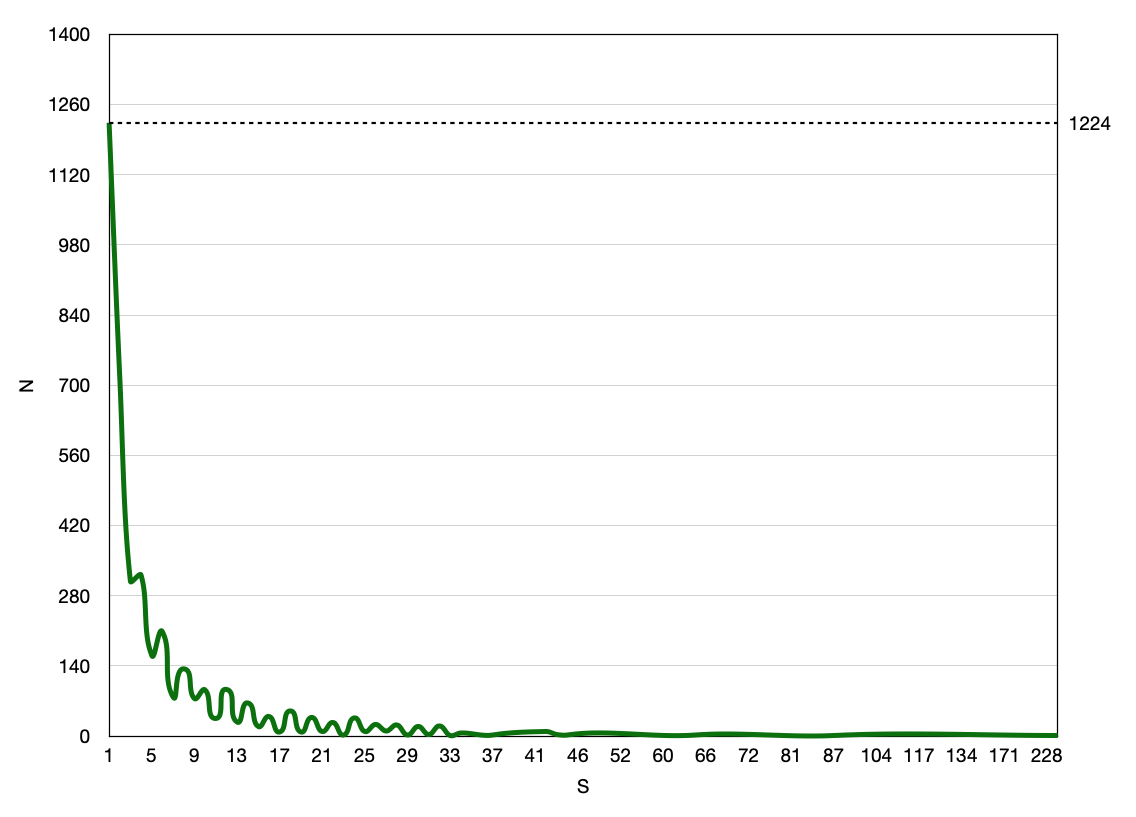
\includegraphics[width=\linewidth]{chapter/city/Number_of_cities_having_given_number_of_sister_cities_according_to_Wikidata,_2020.png}}
}
	\caption{Relation between number of sister cities the city have (S) and number of cities which have this amount of sister cities (N), 2020.}
	\labfig{fig:city_relation_S_N}
\end{marginfigure}

The result of SPARQL query for all cities is shown in \reffig{fig:city_relation_S_N}. The maximum value of N (\num{1224} cities) is observed when S is equal to one, followed by a sharp decrease in the number of cities with an increase in the number of their sister cities. In \reffig{fig:city_ln_relation_S_N} the obtained data is also presented, but on a logarithmic scale. Thus, a little more than four thousand cities (4046 cities) have at least one sister city, of which:

\begin{itemize}
\item 32\% (1314 cities) have relations with more than five cities;
\item 18\% (728 cities) have at least eleven sister cities;
\item 9\% (345 cities) friends with more than twenty cities;
\item 2\% (94 cities) have fifty or more sister cities.
\end{itemize}

\begin{figure*}[h]
{
\setlength{\fboxsep}{0pt}%
\setlength{\fboxrule}{1pt}%
\fcolorbox{gray}{gray}{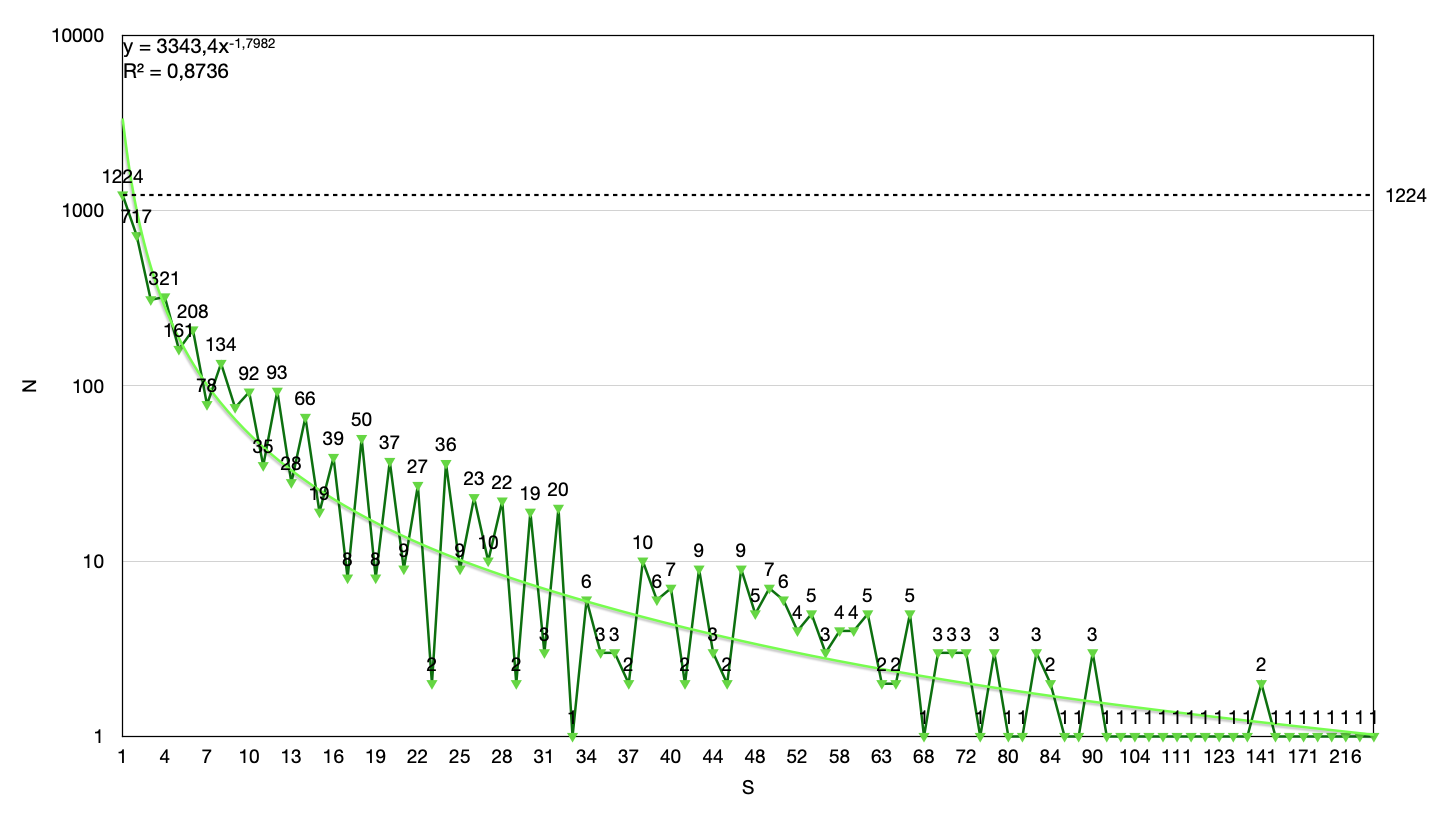
\includegraphics[width=\linewidth]{chapter/city/Logarithm_of_the_number_of_cities_having_given_number_of_sister_cities_according_to_Wikidata,_2020.png}}%
}
  \caption{Relation between number of sister cities the city have (S) and logarithm of the number of cities which have this amount of sister cities (N), 2020.}%
  \labfig{fig:city_ln_relation_S_N}%
\end{figure*}

Based on the constructed trend, it can be concluded that the relation between number of sister cities the city have and number of cities which have this amount of sister cities has a distribution close to a power law.

\begin{lstlisting}[ language=SPARQL, 
                    caption={Number of Russian cities with certain amount of sister cities\\\hspace{\textwidth}
                        The result contains 24 variants of sister city amount in 2020.\\\hspace{\textwidth}
                        SPARQL query: \href{https://w.wiki/m3H}{w.wiki/m3H}
                        },
                    label=lst:city_relation_Russia_S_N,
                    texcl 
                    ]
#defaultView:LineChart                                                   
# Count No. of cities having sisterCount sister cities  
# and number of sister cities themselves
SELECT ?sisterCount (COUNT(?sisterCount) AS ?FreqNSister) WHERE {                                                                                  
	{ # Count sister cities of cities which are ...
		SELECT (COUNT(?sister) AS ?sisterCount) WHERE {    
			{ ?city wdt:P31 wd:Q3957 } UNION # instances of "town"
			{ ?city wdt:P31 wd:Q515 } UNION # OR instances of "city"
			{ ?city wdt:P31 wd:Q1549591 } UNION # OR instances of "big city"
			{ ?city wdt:P31 wd:Q1637706 } # OR instances of "city 1000000+"
			?city wdt:P17 wd:Q159. # belonging to Russia
			?city wdt:P190 ?sister. # with filled property "sister city"
		}
		GROUP BY ?city # Group list by city                             
	}
}
GROUP BY ?sisterCount # Group by number of sister cities
ORDER BY DESC(?sisterCount) # Order by number of sister cities
\end{lstlisting}%

\begin{marginfigure}[-2cm]
{
\setlength{\fboxsep}{0pt}%
\setlength{\fboxrule}{1pt}%
\fcolorbox{gray}{gray}{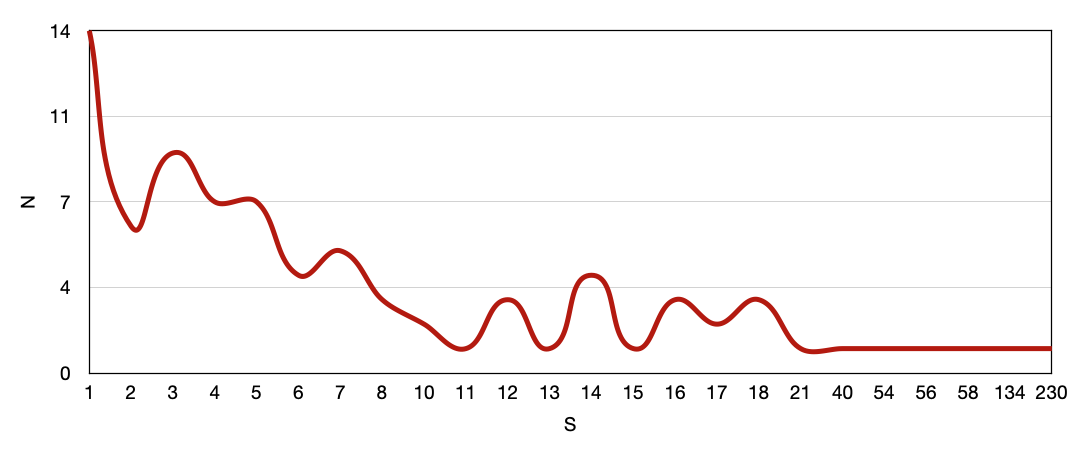
\includegraphics[width=\textwidth]{chapter/city/Number_of_Russian_cities_having_given_number_of_sister_cities_according_to_Wikidata,_2020.png}}%
}
  \caption{Relation between number of sister cities the Russian city have (S) and number of Russian cities which have this amount of sister cities (N), 2020.}%
  \labfig{fig:city_relation_Russia_S_N}%
\end{marginfigure}

The situation with Russian cities is shown in \reffig{fig:city_relation_Russia_S_N}. A little less than a hundred Russian cities (82 cities) have at least one sister city, of which only 48\% (39 cities) are connected with over than five cities.

\subsection{Which country has the most sister cities?}

The SPARQL query for construction a list of countries ordered by number of sister cities is presented below (Listing \ref{lst:countries_sister_cities}). The result of this query is shown in \reffig{fig:Bubble_countries_sister_cities}.

\begin{marginfigure}[2cm]
{
\setlength{\fboxsep}{0pt}%
\setlength{\fboxrule}{1pt}%
\fcolorbox{gray}{gray}{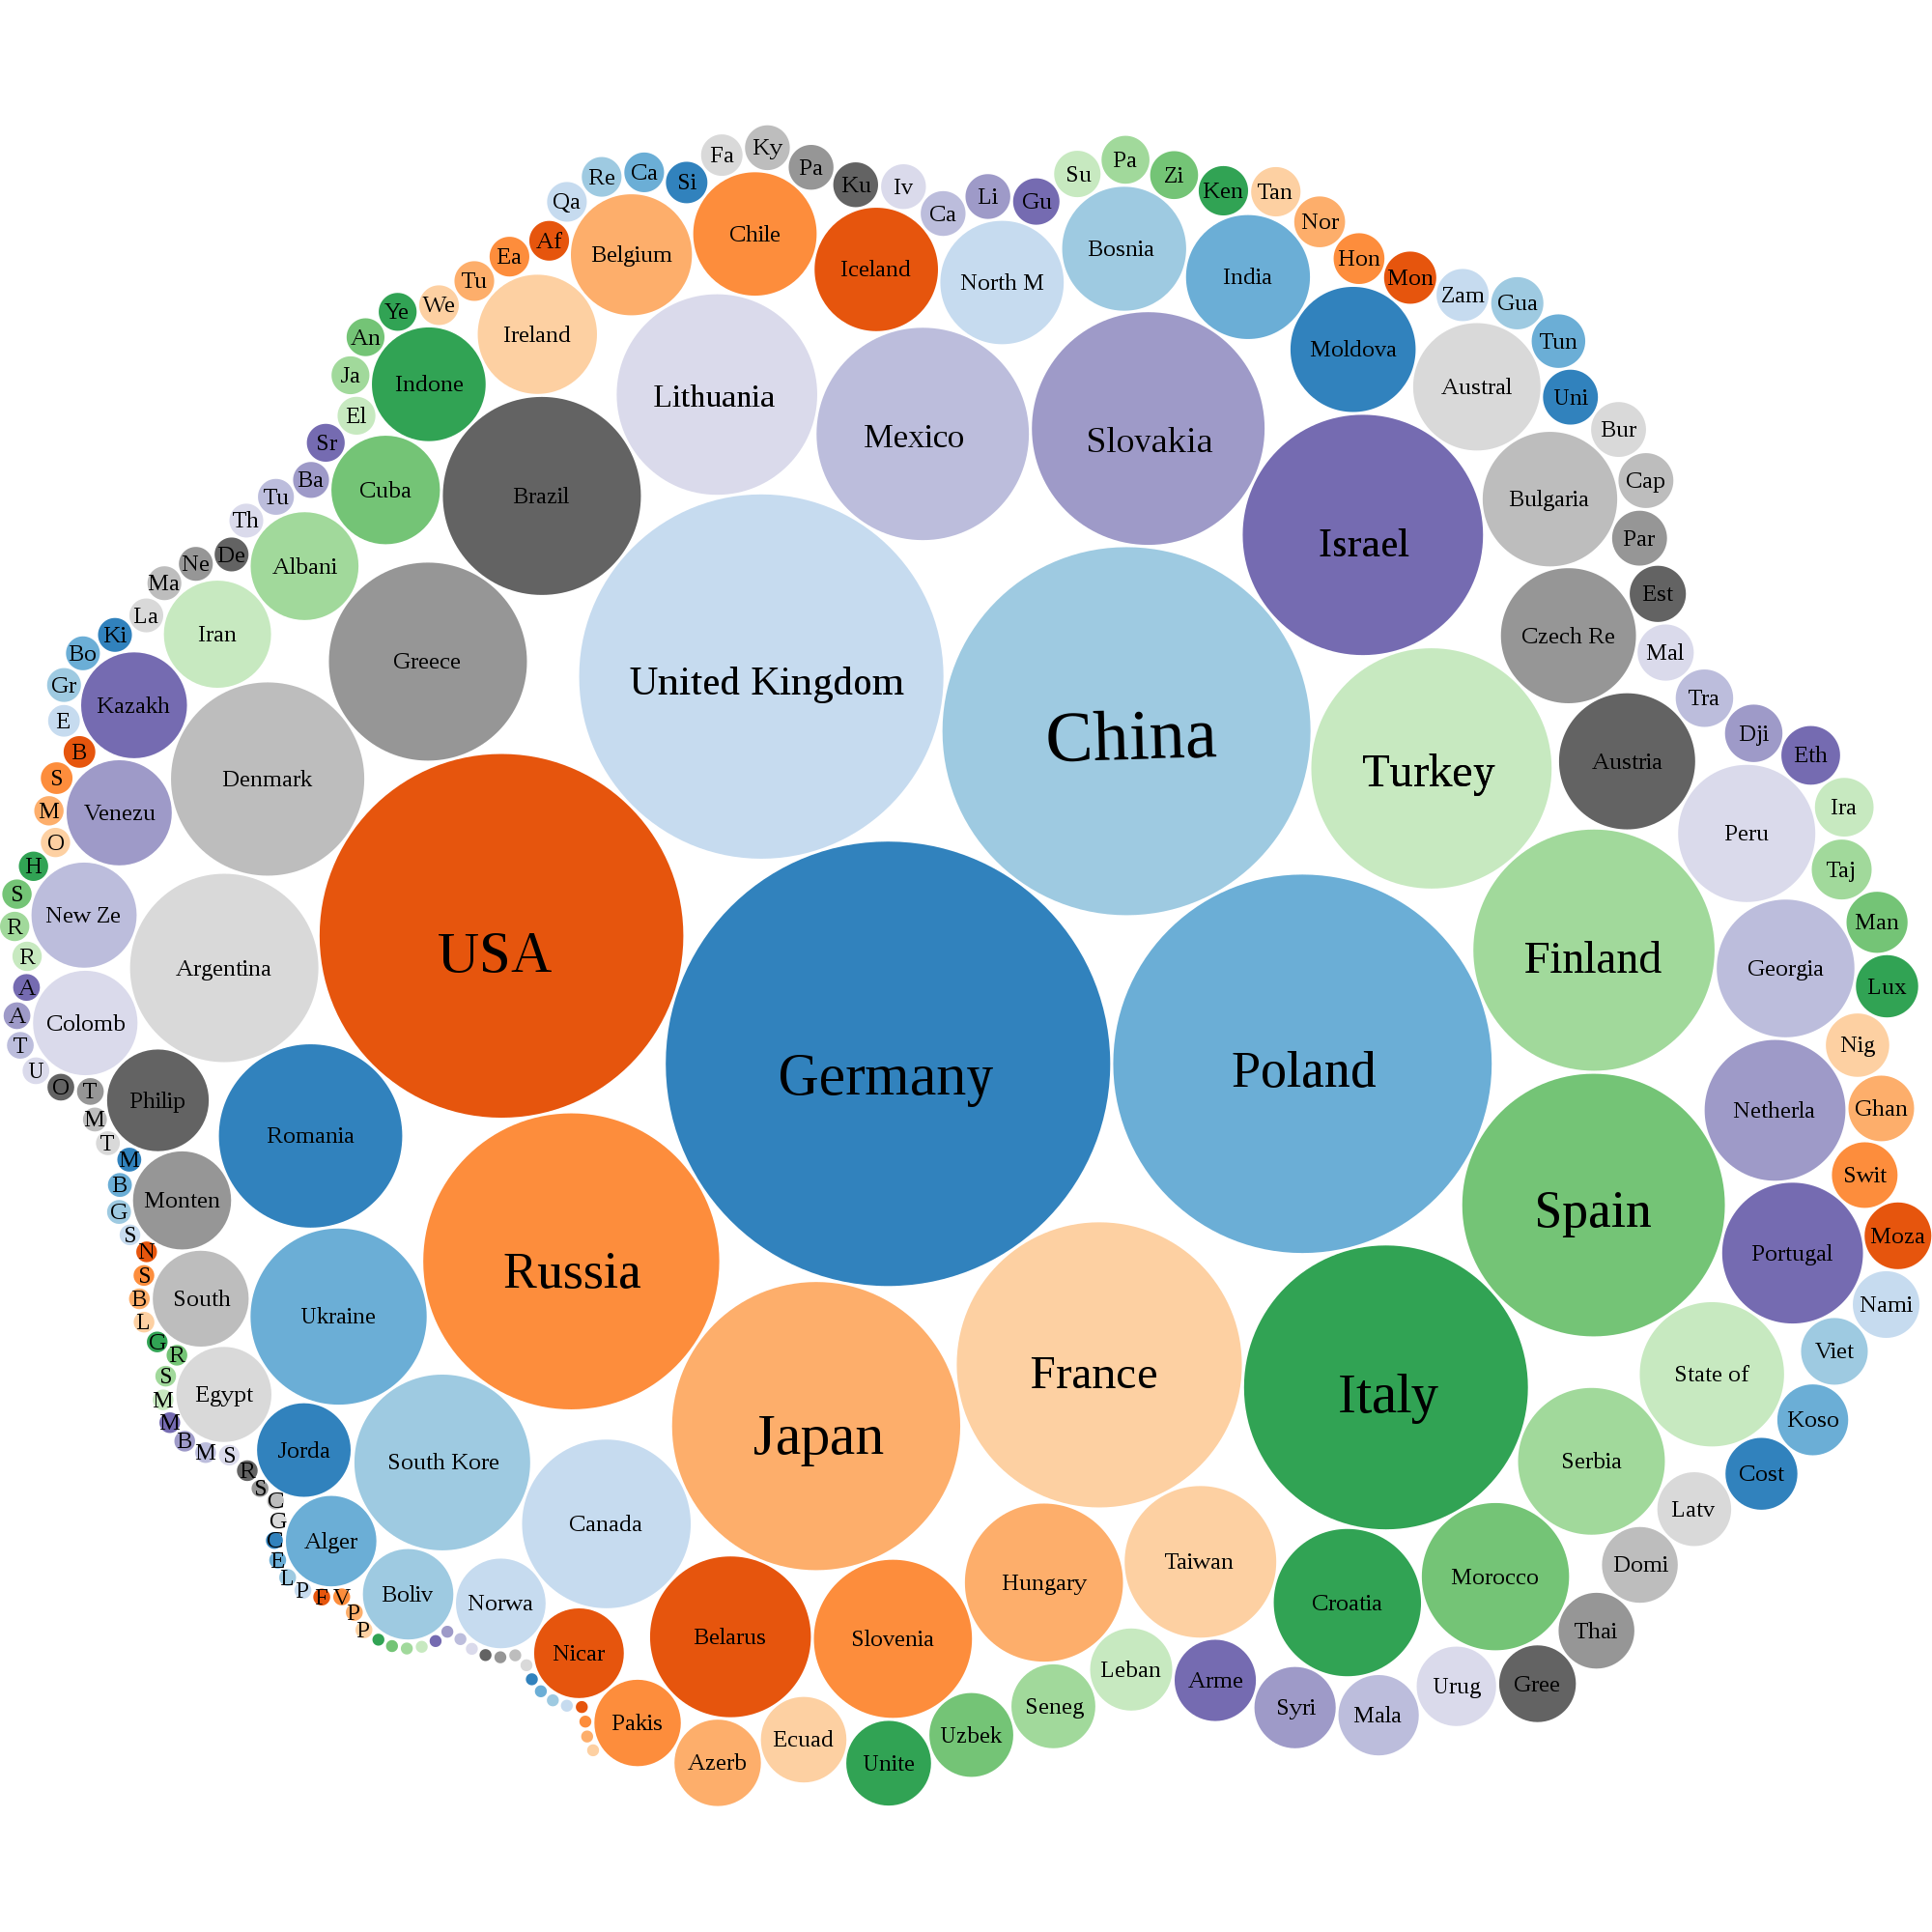
\includegraphics[width=\linewidth]{chapter/city/Bubble_chart_number_of_sister_cities_of_countries_according_to_Wikidata,_2020_(EN).png}}
}
	\caption{Bubble chart by the number of sister cities of countries, 2020.}
	\labfig{fig:Bubble_countries_sister_cities}
\end{marginfigure}

\begin{lstlisting}[ language=SPARQL, 
                    caption={List of countries ordered by number of sister cities\\\hspace{\textwidth}
                        The result contains 208 records in 2020.\\\hspace{\textwidth}
                        SPARQL query: \href{https://w.wiki/m3E}{w.wiki/m3E}
                        },
                    label=lst:countries_sister_cities,
                    texcl 
                    ]
#defaultView:BubbleChart
# Selecting number of distinct sister cities of particular  
# country cities which are ... 
SELECT ?countryLabel (COUNT(?sister) as ?sisterCount) WHERE { 
	SELECT DISTINCT ?countryLabel ?sister WHERE {
		{ ?city wdt:P31 wd:Q3957 } UNION # instances of "town"
		{ ?city wdt:P31 wd:Q515 } UNION # OR instances of "city"
		{ ?city wdt:P31 wd:Q1549591 } UNION # OR instances of "big city"
		{ ?city wdt:P31 wd:Q1637706 }. # OR instances of "city 1000000+"
		?city wdt:P17 ?country. # with filled property "country"
		?city wdt:P190 ?sister. # with filled property "sister city"
		SERVICE wikibase:label { bd:serviceParam wikibase:language "en" }
	}                                 
}
GROUP BY ?countryLabel
ORDER BY DESC(?sisterCount)
\end{lstlisting}%

Germany had the largest number of sister cities (1375 cities) for 2020. The \reftab{tab:germany_sister_cities} shows a list of ten countries that have the largest number of sister cities with Germany (2020). You can get a full list of countries with which Germany has sister cities by running the SPARQL query below (Listing \ref{lst:sister_cities_with_Germany}).

\begin{table}[h]
  \centering
  \fontfamily{ppl}\selectfont
  \begin{tabular}{| c | l | r | r |}
    \toprule
   \# & \multicolumn{1}{ c |}{Country} & \multicolumn{1}{p{0.2\textwidth} |}{\centering Number of sister cities} & \multicolumn{1}{p{0.15\textwidth} |}{\centering \% of total} \\
   \midrule
    1 & \wdqName{France}{142} & 247 & \num{18,0}\% \\
    2 & \wdqName{Germany}{183} & 195 & \num{14,2}\% \\
    3 & \wdqName{United Kingdom}{145} & 120 & \num{8,7}\% \\
    4 & \wdqName{Italy}{38} & 86 & \num{6,3}\% \\
    5 & \wdqName{Poland}{36} & 81 & \num{5,9}\% \\
    6 & \wdqName{United States of America}{30} & 60 & \num{4,4}\% \\
    7 & \wdqName{Austria}{40} & 41 & \num{3,0}\% \\
    8 & \wdqName{Russia}{159} & 39 & \num{2,8}\% \\
    9 & \wdqName{Hungary}{28} & 39 & \num{2,8}\% \\
    10 & \wdqName{Belgium}{31} & 33 & \num{2,4}\% \\
    \bottomrule  \end{tabular}%
  \caption{List of countries having the largest number of sister cities with Germany cities, 2020.}
  \labtab{tab:germany_sister_cities}
  %\zsavepos{pos:normaltab}
\end{table}

\begin{lstlisting}[ language=SPARQL, 
                    caption={List of countries having sister cities with Germany cities \\\hspace{\textwidth}
                        The result contains 93 records in 2020.\\\hspace{\textwidth}
                        SPARQL query: \href{https://w.wiki/m3A}{w.wiki/m3A}
                        },
                    label=lst:sister_cities_with_Germany,
                    texcl 
                    ]
# Selecting number of distinct particular country sister cities  
# of cities which are ...
SELECT ?country ?countryLabel 
				(COUNT(DISTINCT ?sister) as ?sisterCount) WHERE {                                                          
	{ ?city wdt:P31 wd:Q3957 } UNION # instances of "town"
	{ ?city wdt:P31 wd:Q515 } UNION # OR instances of "city"
	{ ?city wdt:P31 wd:Q1549591 } UNION # OR instances of "big city"      
	{ ?city wdt:P31 wd:Q1637706 }. # OR instances of "city 1000000+"
	?city wdt:P17 wd:Q183. # belonging to Germany  
	?city wdt:P190 ?sister. # with filled property "sister city"
	?sister wdt:P17 ?country. # with filled property "country"
	SERVICE wikibase:label { bd:serviceParam wikibase:language "en" }
}
GROUP BY ?country ?countryLabel
ORDER BY DESC(?sisterCount)
\end{lstlisting}%

\subsection{Closest neighbours of Russia}

The SPARQL query for construction a list of countries with which Russia has sister cities is presented below (Listing \ref{lst:countries_sister_cities_with_Russia}). The result of this query is shown in \reffig{fig:Bubble_countries_sister_cities_with_Russia}.

\begin{marginfigure}[2cm]
{
\setlength{\fboxsep}{0pt}%
\setlength{\fboxrule}{1pt}%
\fcolorbox{gray}{gray}{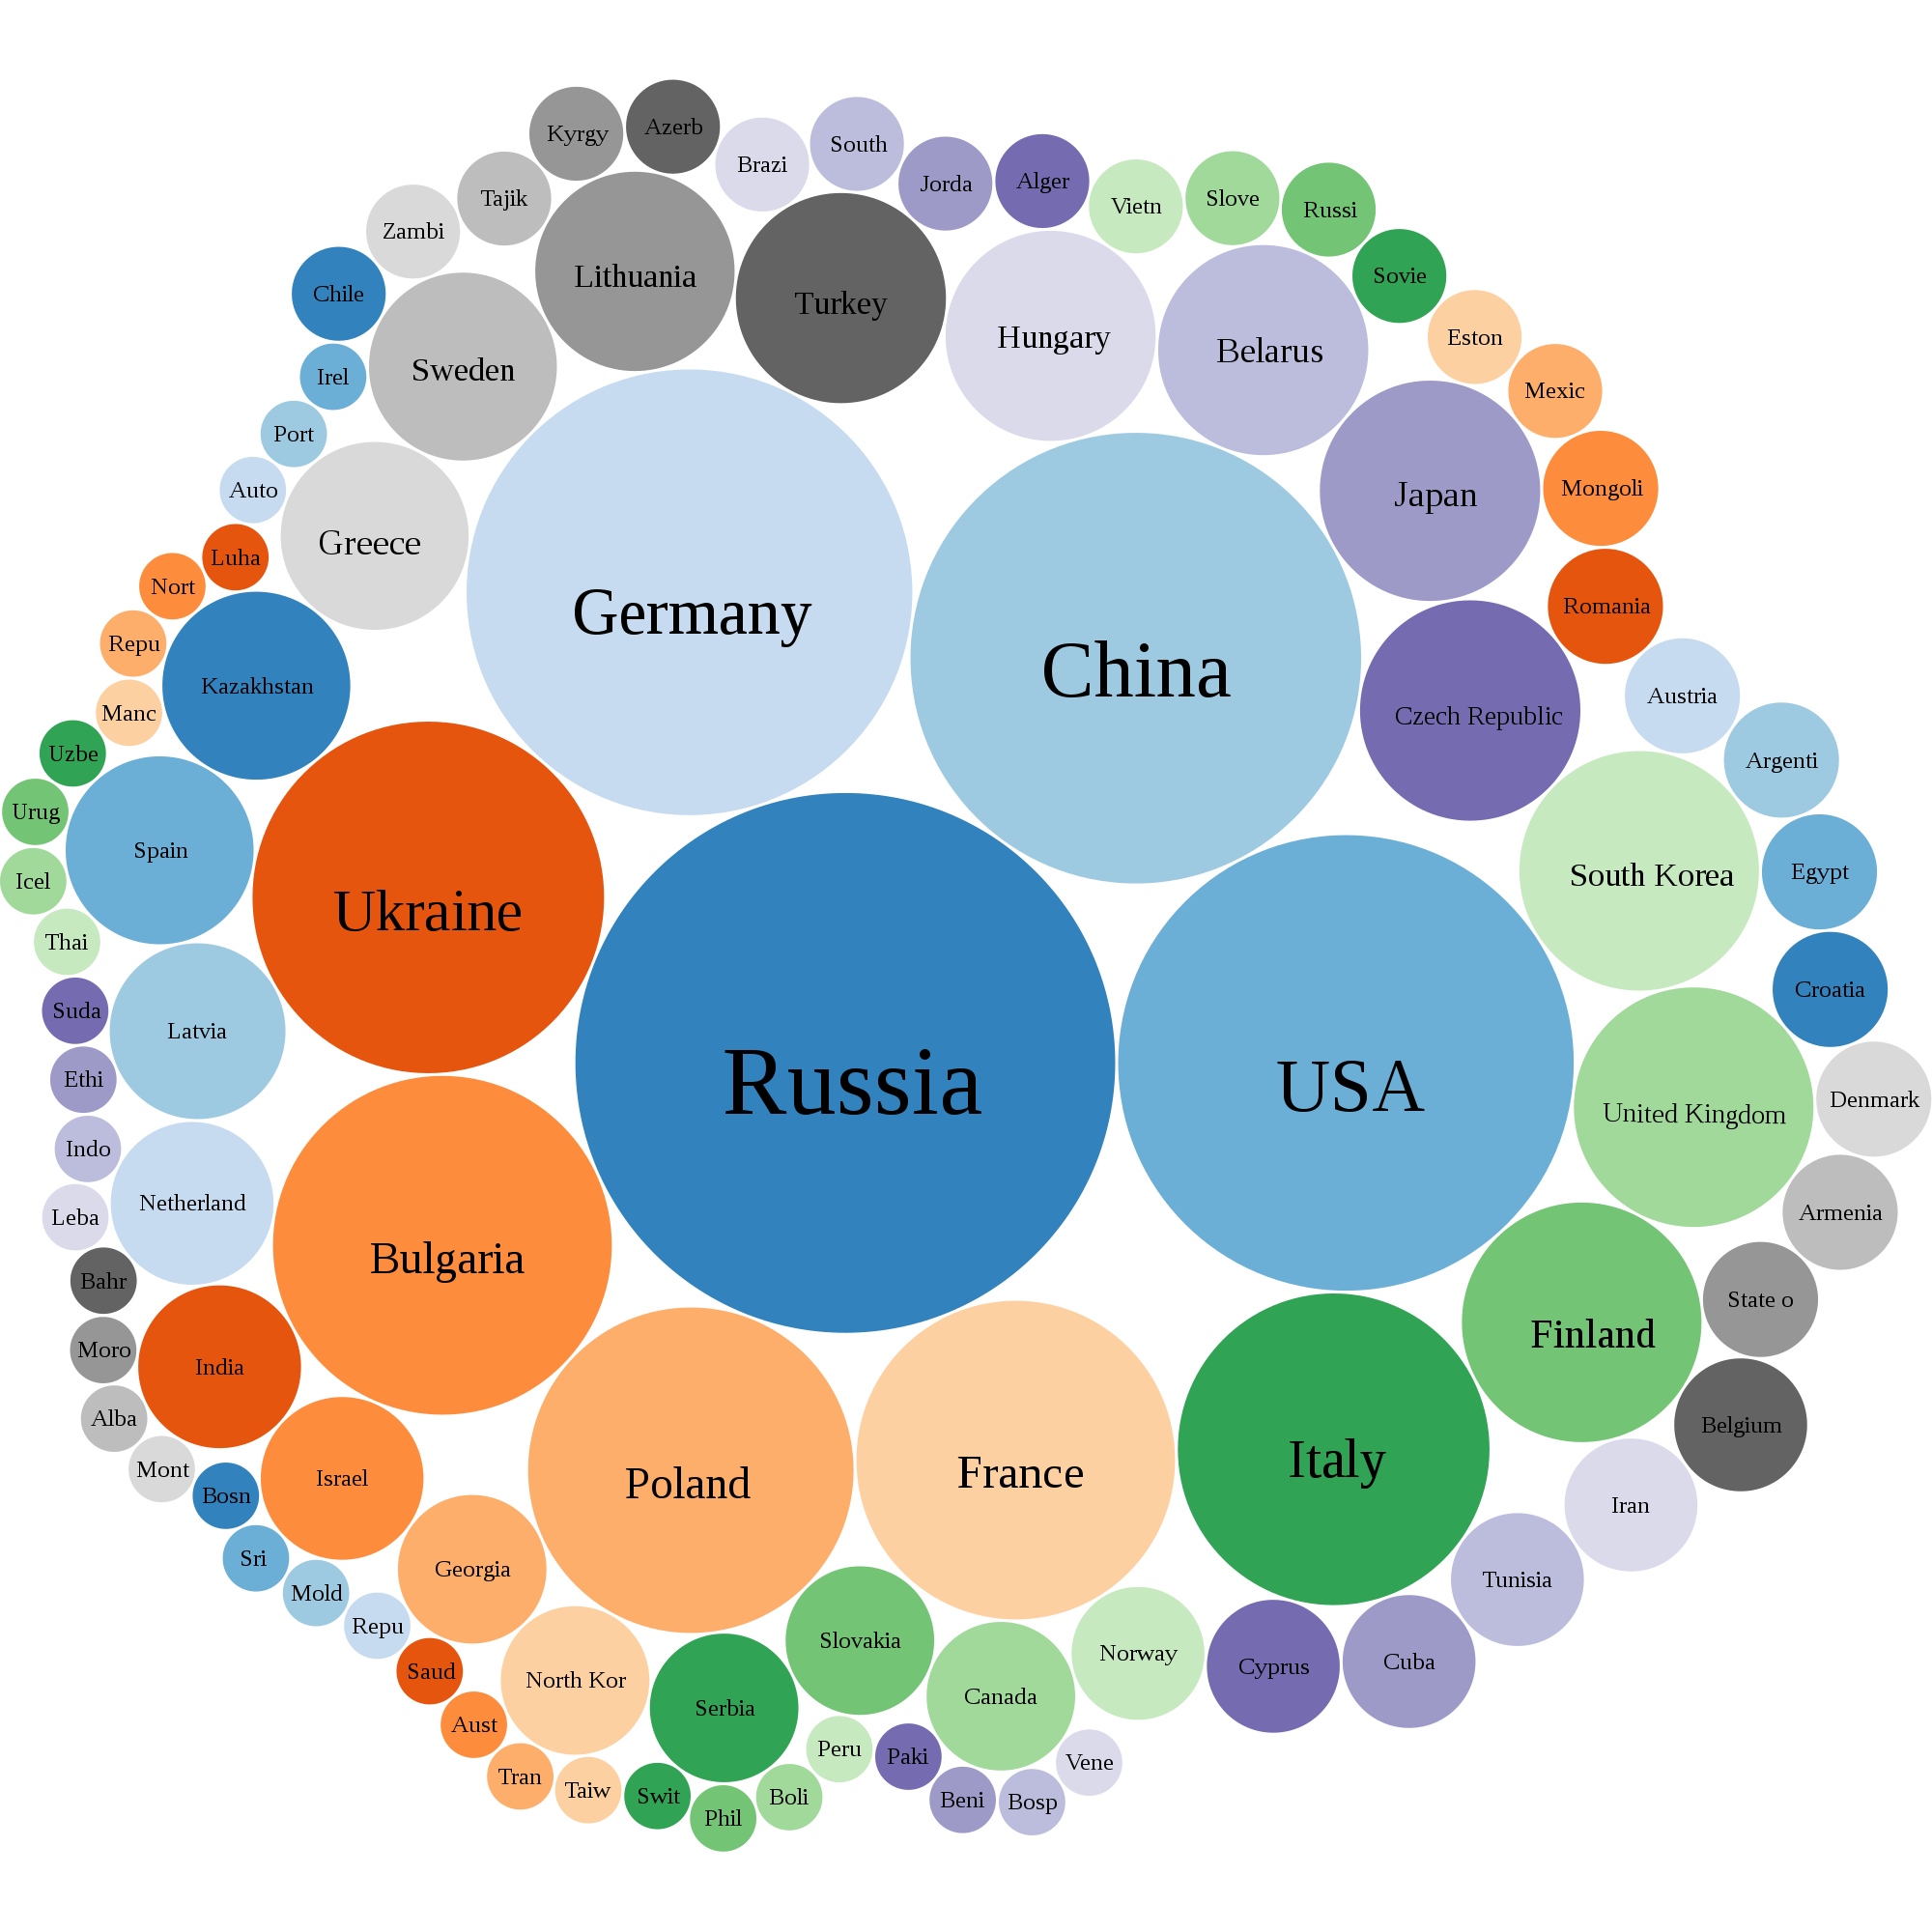
\includegraphics[width=\linewidth]{chapter/city/Bubble_chart_number_of_sister_cities_with_Russia_of_countries_according_to_Wikidata,_2020_(EN).png}}
}
	\caption{Bubble chart by the number of Russian sister cities with countries, 2020.}
	\labfig{fig:Bubble_countries_sister_cities_with_Russia}
\end{marginfigure}

\begin{lstlisting}[ language=SPARQL, 
                    caption={Closest neighbours of Russia\\\hspace{\textwidth}
                        The result contains 96 records in 2020.\\\hspace{\textwidth}
                        SPARQL query: \href{https://w.wiki/m37}{w.wiki/m37}
                        },
                    label=lst:countries_sister_cities_with_Russia,
                    texcl 
                    ]
#defaultView:BubbleChart
# Selecting number of distinct particular country sister cities 
# of cities which are ...
SELECT ?country ?countryLabel 
				(COUNT(DISTINCT ?sister) as ?sisterCount) WHERE {                                                
	{ ?city wdt:P31 wd:Q3957 } UNION # instances of "town"
	{ ?city wdt:P31 wd:Q515 } UNION # OR instances of "city"
	{ ?city wdt:P31 wd:Q1549591 } UNION # OR instances of "big city"
	{ ?city wdt:P31 wd:Q1637706 }. # OR instances of "city 1000000+"                                 
	?city wdt:P17 wd:Q159. # belonging to Russia
	?city wdt:P190 ?sister. # with filled property "sister city"
	?sister wdt:P17 ?country. # with filled property "country"
	SERVICE wikibase:label { bd:serviceParam wikibase:language "en" }
}
GROUP BY ?country ?countryLabel
ORDER BY DESC(?sisterCount)
\end{lstlisting}%

Russia has more than twenty sister cities with countries such as United States of America (47), China (46), Germany (45), Ukraine (28), Bulgaria (26), Poland (24), France (23) and Italy (22).

%%%%%%%%%%%%%%%%%%%%%%%%%%%%%%%%%%%%%%%%%%%%%%%%%%%%%%%
\section{Wikidata completeness and disadvantages}

City is a type of human settlement with people not occupied with agriculture. At the same time, different countries use different criteria when assigning city status to settlements, the main of which is population. Some countries don't define a term "city" at all. So, in France, only one geographic unit of this kind is used — a commune, regardless of the number of people living in it and the type of their activity. Therefore, it can be difficult to clearly determine which settlement is classified as a city and which is not.

In practice, some Wikidata objects can simultaneously be instances of different types of cities. For example, \wdqName{Shanghai}{8686} is assigned to three objects under study:  \wdqName{city}{515}, \wdqName{big city}{1549591}, \wdqName{city with millions of inhabitants}{1637706}. It is easy to guess that such multiple assignment affects the results of SPARQL queries, in particular, using the \href{https://en.wikibooks.org/wiki/SPARQL/UNION}{UNION} construction. This can be verified by running, for example, SPARQL query for finding instances of different types of cities (Listing \ref{lst:different_city_types}). \wdqName{Shanghai}{8686} is found in the results for three times.

Wikidata has an inheritance mechanism expressed in the  \href{https://www.wikidata.org/wiki/Property:P279}{subclass of} property. This mechanism consists in the fact that if an object is an instance of \wdqName{big city}{1549591}, then it is also an instance of \wdqName{city}{515}, since \wdqName{big city}{1549591} is a subclass of \wdqName{city}{515}. Thus, the situation described above with \wdqName{Shanghai}{8686} can be resolved by leaving only one class — \wdqName{city with millions of inhabitants}{1637706}. It should be noted that replacing a \href{https://en.wikibooks.org/wiki/SPARQL/UNION}{UNION} construction (Listing  \ref{lst:example_union_city}) with a subclassing construction (Listing \ref{lst:example_subclasses_city}) is not equivalent. \wdqName{Shanghai}{8686}, considered earlier, can be found four times in the new query results. The fact is that in addition to some of the objects under study, there are other classes inherited from \wdqName{city}{515}. For example, \wdqName{lost city}{2974842}, \wdqName{free imperial city}{57318}, \wdqName{autonomous city}{1094397} and even \wdqName{ideal city}{1656724}.


\begin{lstlisting}[ language=SPARQL, 
                    caption={Example of UNION construction\\\hspace{\textwidth}
                        SPARQL query: \href{https://w.wiki/m34}{w.wiki/m34}
                        },
                    label=lst:example_union_city,
                    texcl 
                    ]
SELECT ?city ?cityLabel WHERE { # Selecting items which are ...
	{ ?city wdt:P31 wd:Q515 } UNION # instances of "city"            
	{ ?city wdt:P31 wd:Q1549591 } UNION # instances of "big city"               
	{ ?city wdt:P31 wd:Q1637706 } 	# instances of "city 1000000+"
	SERVICE wikibase:label { bd:serviceParam wikibase:language "en" }
}
\end{lstlisting}%


\begin{lstlisting}[ language=SPARQL, 
                    caption={Example of construction with subclasses\\\hspace{\textwidth}
                        SPARQL query: \href{https://w.wiki/m32}{w.wiki/m32}
                        },
                    label=lst:example_subclasses_city,
                    texcl 
                    ]
SELECT ?city ?cityLabel WHERE { # Selecting items which are ...
	?city wdt:P31/wdt:P279* wd:Q515 # instances of "city" subclasses
	SERVICE wikibase:label { bd:serviceParam wikibase:language "en" }
}
\end{lstlisting}%

Also, probably with ambiguity in the criteria for assigning city status, subclasses were created for specific countries — \wdqName{city in Chile}{25412763}, \wdqName{city in Cyprus}{29556224}, \wdqName{city of Japan}{494721} and so on. This tendency was not spared by the cities of Russia, which could be noticed when comparing the results of a SPARQL query to find instances of the "city" object (Listing \ref{lst:city}). At the moment, most of them belong to the \wdqName{city/town}{7930989} class.

According to the \href{http://www.gks.ru/free\_doc/new\_site/perepis2010/croc/Documents/Vol1/pub-01-03.pdf}{Russian Census (2010)} and the \href{https://rosstat.gov.ru/free\_doc/new\_site/population/demo/perepis\_krim/KRUM\_2015.pdf}{Crimean Federal District Census (2014)}, the total number of Russian cities was \num{1117} in 2014. All cities in Russia have an article in both Russian and English Wikipedia.

Number of Wikidata elements which are Russian cities equals to \href{https://w.wiki/ngM}{\num{1126}}. It can be assumed that Wikidata completely covers, at least, Russian cities.

%%%%%%%%%%%%%%%%%%%%%%%%%%%%%%%%%%%%%%%%%%%%%%%%%%%%%%%
\section{Tasks}
\begin{enumerate}
\item Construct a graph of Russian sister cities.
\item Get list of Russian cities situated beyond the Arctic circle.
\item On which river in Russia is the largest number of cities located?
\end{enumerate}